% !TEX root = quickstep.tex

\section{Scheduling \& Execution} \label{query-exec}
In this section, we describe how the design of the query processing engine in \Quickstep\ achieves three key objectives. First, we believe that separating the control flow and the data flow involved in query processing allows for greater flexibility in reacting to runtime conditions and facilitates maintainability and extensibility of the system. To achieve this objective, the engine separates responsibilities between a scheduler, which makes work scheduling decisions, and workers that execute the data processing kernels (cf. Section~\ref{sec:threading-model}).

Second, to fully utilize the high degree of parallelism offered by modern processors, \Quickstep\ complements its block-based storage design with a work order-based scheduling model (cf. Section~\ref{scheduler}) to obtain high intra-query and intra-operator parallelism.

Finally, to support diverse scheduling policies for sharing resources (such as CPU and memory) between concurrent  queries, the scheduler design separates the choice of policies from the execution mechanisms (cf. Section~\ref{sec:scheduler-policy-vs-mechanism}).

%The scheduler in Quickstep is a crucial component and we describe it in this section. Query execution in \Quickstep\ leverages the block-based storage manager design described in Section~\ref{storage-manager}, and uses a workflow-based query execution paradigm. In \Quickstep, query execution involves generating a series of \textit{work orders} that are then executed by workers. A work order largely corresponds to applying some operation on a block of input tuples (Section~\ref{scheduler} below has more details).

%\subsection{Operator Algorithms} \label{operators}
%In this section, we briefly describe the operator algorithms that are currently implemented in \Quickstep.
%
%\Quickstep\ has a novel implementation of the selection operator where the operator can decide, on a block-by-block basis, what algorithm to use to apply the selection operation. When applying a predicate, the ``micro-optimizer'' (see Section~\ref{vectorization}) may choose to evaluate some or all of the predicate using a fast path like an index lookup
%%(using a BitWeaving or CSB+-Tree index),
%or a binary search on a sorted column in a column-store. If no fast-path is available, the system falls back to iterating over the tuples in a block and evaluating the predicate(s) in a vectorized fashion. The next step in evaluating the selection operation is to materialize the expressions in the projection list (again using vectorized column-at-a-time execution), and bulk-inserting the resultant tuples into a temporary in-memory block for consumption by other operators. In the common case when the projection simply copies column values as is from the input, the expression evaluation component is skipped entirely and data is directly copied from one block into another.
%
%\subsubsection{Hash Join} \label{sec:inline-tuples}
%\Quickstep\ implements a traditional hash join algorithm consisting of a build phase and a probe phase. These phases are implemented as separate operators. The build hash table operator reads blocks of the build relation, and builds a single cache-efficient hash table in memory using the join predicate as the key (borrowing the ideas proposed in~\cite{BlanasLP11}). The probe hash table operator reads blocks of the probe relation, probes the hash table, and materializes joined tuples into in-memory blocks for consumption by other operators, just like the selection operator does. Both the build and probe operators take advantage of block-level parallelism, and use a latch-free concurrent hash table to allow multiple workers to proceed at the same time.
%
%For non-equijoins, \Quickstep\ uses a block-nested loops join algorithm.  %(which also allows a ``residual'' filter predicate to be used with a hash-join to filter joined tuple pairs on a non-equijoin predicate in addition to the equality predicate evaluated by hashing). %Note that the resize operation of hash table is not lock-free.
%
%The basic hash join operator has also been adapted to support left outer join, left semijoin, and antijoin operators.
%
%%An important optimization is used for the hash table, which we describe next.
%
%%\textbf{Inlining tuples in a hash table: } An important issue, which hasn't received much attention in the literature, is how to deal with the payload associated with the entries in a hash table, when used for join evaluation. The common approach is to store in the hash table the key(s) of the build-side tuple along with a pointer/reference to the build tuple. However, this approach may incur a large overhead in retrieving the build tuples when the join is ready to materialize its output and when the result join tuple has build-side attributes that are not part of the join key(s).
%
%%An alternative approach is to store the required build-side attributes (in a row-store format) in the hash table itself. This approach avoids incurring the potentially expensive operation of fetching the build tuple, which is most likely no longer in the processor caches when it is retrieved. (The reason for this behavior is because the task of building the hash table was followed by a batch-based probing of the hash table using the tuples in the current probe block. The probe operation will have likely wiped out the build tuples from the cache.) However, this inlining approach imposes an additional space overhead on the hash table, as the hash table could now be potentially larger. \Quickstep\ uses a simple rule that is based on examining the size of the in-lined tuple and the resulting size of the hash bucket. If this size is smaller than the processor cache line size, then inlining is turned on.
%
%\subsubsection{Aggregation}
%%For aggregation without GROUP BY, the aggregate operator reads blocks of the input relation and generates work orders per block that compute the aggregates local to their assigned block.
%For aggregation without \texttt{GROUP BY}, the operator computes local aggregates for each input block.
%These local aggregates are later merged with the global aggregates for the entire query.
%%For aggregation with GROUP BY, the operator generates work orders per block that together build a (latch-free) hash table of aggregation handles in parallel using the grouping columns as the key.
%For aggregation with \texttt{GROUP BY}, the operator builds a global latch-free hash table of aggregation handles in parallel, using the grouping columns as the key.
%%After processing all the blocks in the input relation, a work order iterates through the hash table to output the grouping keys and their corresponding aggregates, or just the aggregates in the case of aggregation without GROUP BY.
%% Note that this final phaseof iterating through the hash table and output tuples can be parallelized further by
%% assigning parts of the hash table to individual work orders.
%
%\subsubsection{Sort and Top-K}
%\Quickstep\ employs a two-phase algorithm for sorting and top-K operators. These phases are implemented as separate operators. In the first phase, each block of the input relation is sorted in-place, or copied to a single temporary sorted block. This phase is similar to the run generation phase of the traditional external sort. In the second phase, runs of sorted blocks are merged to produce a fully sorted output relation.

\subsection{Threading Model} \label{sec:threading-model}
The \Quickstep\ execution engine consists of a single \textit{scheduler} thread and a pool of \textit{workers}.
The scheduler thread uses the query plan to generate and schedule work for the workers.
When multiple queries are concurrently executing in the system, the scheduler is responsible for enforcing resource allocation policies across concurrent queries and controlling query admittance under high load.
Furthermore, the scheduler monitors query execution progress, enabling status reports as illustrated in Section~\ref{sec:progress-monitoring}.

The workers are responsible for executing the relational operation tasks that are scheduled.
Each worker is a single thread that is pinned to a CPU core (possibly a virtual core), and there are as many workers as cores available to \Quickstep.
The workers are created when the Quickstep process starts, and are kept alive across query executions, minimizing query initialization costs.
The workers are stateless; thus, the worker pool can \textit{elastically} grow or shrink dynamically. %at any time in the database process' runtime.
%It is possible to \textit{elastically} add new workers to the pool while a query is under execution, to provide more parallelism.
%Workers are always stateless, so the scheduler can terminate them either at process termination, after all queries have been completed or cancelled, or even mid-query, in order to react to changes in resource availability.
%This property of ``elasticity'' is illustrated in Section~\ref{sec:expt:elasticity}.
% The elasticity comment is a left over from the previous versions of this paper.
%\reminder{I'm not sure what poison work orders do. Do they terminate the threads? If so, why would we do that to abort a query?}

%The unit of work scheduled by the scheduler is called a \textit{work order}, and is described in the next section.

%The \Quickstep\ execution engine uses two kinds of execution threads, namely \textit{foreman} and \textit{worker} threads.
%
%\textit{Worker threads} execute work orders produced by physical relational operators. The \textit{foreman thread} makes decisions about scheduling the work orders to the Worker threads.
%%The current execution engine allows a single query to be controlled by a single foreman thread.
%All worker threads are stateless. They simply keep executing work orders in a loop. A worker thread can be terminated by sending a special \textit{poison work order}. The work order termination method can then be used to gracefully terminate the \Quickstep\ process, or to abort a query (for example, in response to the client issuing a query cancellation command). %Concurrent queries are supported, and a foreman thread is spawned for every new query that arrives into the system.
%
%To minimize the thread initialization costs, all the Worker threads are created when the \Quickstep\ process is started, and they stay alive until the \Quickstep\ process terminates.
%However, since workers are stateless, it is easy to add or remove them, even mid-query.
%
%All worker threads can be pinned to CPU cores to avoid migration costs when the operating system (OS) decides to move a thread from one CPU core to another.

\subsection{Work Order-based Scheduler}\label{scheduler}
The \Quickstep\ scheduler divides the work for the entire query into a series of \textit{work orders}. In this section,
%we describe this work order-based scheduler.
we first describe the work order abstraction and provide a few example work order types. Next, we explain how the scheduler generates work orders for different relational operators in a query plan, including handling of pipelining and internal memory management during query execution.
%We also explain how the \Quickstep\ scheduler handles query execution aspects such as pipelining and internal memory management during a query execution.

\begin{figure}
\centering
   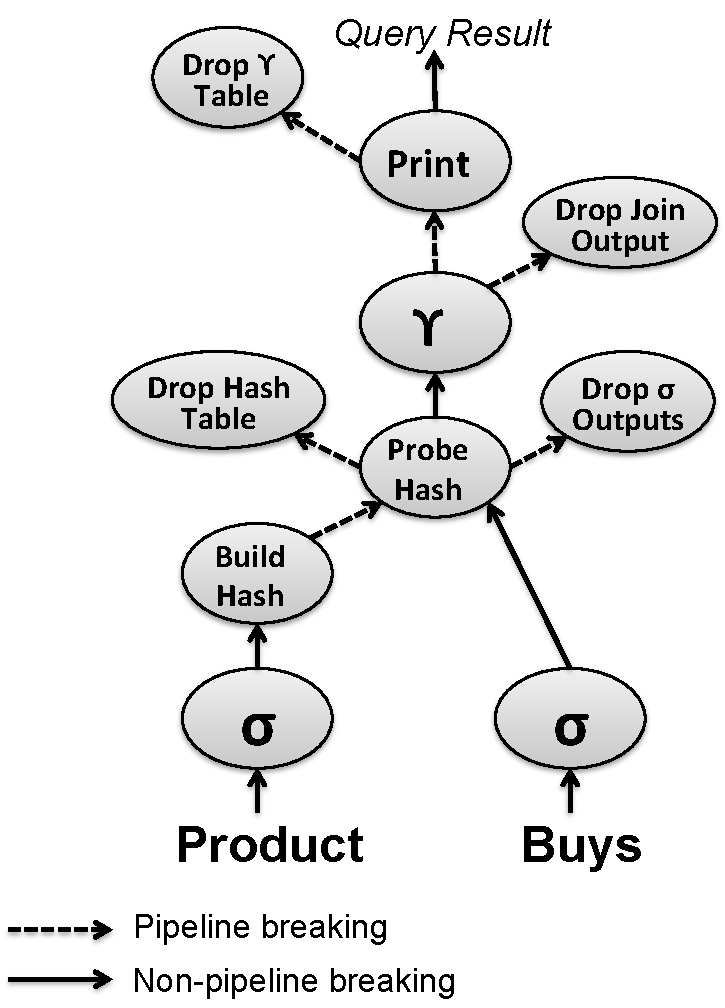
\includegraphics[width=.7\columnwidth]{pictures/physical-plan.pdf}
   \caption{\textbf{Plan DAG for the sample query}}
   \label{fig-dag}
\end{figure}

The optimizer sends to the scheduler an execution query plan represented as a directed acyclic graph (DAG) in which each node is a relational operator. Figure~\ref{fig-dag} shows the DAG for the example query shown below. Note that the edges in the DAG are annotated with whether the producer operator is blocking or permits pipelining.
%consumer operator is blocked on the output produced by the producer operator, or whether data pipelining is allowed between neighboring operators.

%The optimal query plan that is produced by the optimizer is converted to a DAG of operators.
%This DAG representation of the query is then sent to the scheduler.

\begin{lstlisting}[language=SQL,upquote=true,
basicstyle=\ttfamily\small,
showstringspaces=false,
keywordstyle=\color{cardinal}\bfseries,
emphstyle=\color{bondiblue}\bfseries,
stringstyle=\color{bondiblue}\bfseries,
emph={SUM}]
  SELECT SUM(sales)
  FROM   Product P NATURAL JOIN Buys B
  WHERE  B.buy_month = 'March'
  AND    P.category = 'swim'
\end{lstlisting}


\subsubsection{Work Order}

%Each relational operator presents the work that needs to be done to execute the query using \textit{work orders}.
A \textit{work order} is a unit of intra-operator parallelism for a relational operator. Each relational operator in Quickstep describes its work in the form of a set of work orders, which contains references to its inputs and all its parameters.
%For concreteness, we describe some sample work orders for few relational operators.
For example, a \textit{selection work order} contains a reference to its input relation, a filtering predicate, and a projection list of attributes (or expressions) as well as a reference to a particular input block. A selection operator generates as many work orders as there are blocks in the input relation. Similarly, a \textit{build hash work order} contains a reference to its input relation, the build key attribute, a hash table reference, and a reference to a single block of the input build relation to insert into the hash table.

\subsubsection{Work Order Generation and Execution}
%We now describe the work orders generation for a given query plan.

The scheduler employs a simple DAG traversal algorithm to activate nodes in the DAG.
An active node in the DAG can generate \textit{schedulable} work orders, which can be fetched by the scheduler.
In the example query, initially, only the Select operators (shown in Figure~\ref{fig-dag} using the symbol $\sigma$) are active. Operators such as the probe hash and the aggregation operations are initially inactive as their blocking dependencies have not finished execution.
The scheduler begins executing this query by fetching work orders for the select operators. Later, other operators will become active as their dependencies are met, and the  scheduler will fetch work orders from them.
% and they generate work orders -- one for each input block from both input relations.

The scheduler assigns these work orders to available workers, which then execute them. All output is written to temporary storage blocks. After executing a work order, the worker sends a completion message to the scheduler, which includes execution statistics that can be used %by the scheduler
to analyze the query execution behavior.
%The scheduler also relays references to temporary blocks to the next operator in the pipeline.

% which involves the following steps: reading the input block, evaluating the predicate over the block, and writing its output to another block. As noted earlier, the predicate evaluation method for different blocks may be different, subject to their layout, availability of indexes inside the block etc. The complexity of predicate evaluation is abstracted within a block (cf. Section~\ref{block-structure}), and the worker thread and work order code need not know anything about it. As noted in Section~\ref{vectorization}, at run-time each block can decide how to evaluate the predicates. This run-time micro-optimizer picks the physical plan with the lowest estimated cost to evaluate a predicate within each block (possibly using different techniques for different parts of a complex predicate tree). Currently, this micro-optimizer simply employs a pre-defined order of preference for different applicable access paths, but we plan to add basic statistics and selectivity estimation in the future.

\subsubsection{Implementation of Pipelining}
%We now explain how pipelining is implemented in the work order based execution framework.

%Note that in the example query, the hash table is built on the output of the select operator on the Product table.
%The edge connecting the Select operator and the build hash operator allows for \textit{ pipelining}.
%As soon as a filled block of output from an upstream operator (the Select operator in this case) is available, it is streamed to its consumer operator (the build hash operator).
%As soon as some input is available, a work order is created which can then be scheduled by the scheduler.

%The Probe hash work order execution involves checking the hash table for match(es) and writing them to temporary output block(s).
In our example DAG (Figure~\ref{fig-dag}), the edge from the Probe hash operator to the Aggregate operator allows for data pipelining.
As described earlier, the output of each probe hash work order is written in some temporary blocks.
Fully-filled output blocks of probe hash operators can be streamed to the aggregation operator (shown using the symbol $\gamma$ in the figure).
The aggregation operator can generate one work order for each streamed input block that it receives from the probe operator, thereby achieving pipelining.

The design of the Quickstep scheduler separates control flow from data flow.
The control flow decisions are encapsulated in the work order scheduling policy.
This policy can be tuned to achieve different objectives, such as aiming for high performance, staying with a certain level of concurrency/CPU resource consumption for a query, etc.
In the current implementation, the scheduler \textit{eagerly} schedules work orders as soon as they are available.
%Multiple policies are supported including a priority-based policy. With a priority-based policy, work orders from high-priority queries are schedule more frequently. We illustrate this aspect further in Section~\ref{sec:expt:elasticity}. %For the discussion below, we assume a simple fair policy.

%Furthermore, in the current implementation, work orders are executed in a FIFO order. (Clearly, there are future opportunities for exploring other scheduling policies. The key point is that by separating the scheduling policy from the scheduling mechanism, \Quickstep\ has a design that allows for easily varying the scheduling policy, and hence the overall system behavior.)

%Returning to Figure~\ref{fig-dag}, to begin the Probe phase of the Hash Join, the building of the hash table must be complete (note the pipeline-breaking dependency between the Probe and the Build operator). After the build operator has completed, the scheduler is free to schedule a work order for each full block of tuples that is produced by the Select operator on the Buys table. We have a mechanism where the work orders completion triggers a signal to the scheduler indicating that a block is partially full. This mechanism ensures that if a single Selection work order produces a partially filled block, then a handle to that partially filled block is  available to another Selection work order that runs later. Thus, we minimize internal fragmentation for intermediate blocks. % between operators.
%don't have internal fragmentation for blocks as the query execution moves through the DAG.

%select work order on the buys table or it can wait until the building of hash table is over. The select work orders on buys get executed similarly as the select work orders on the Product table. There's one select work order per input block of Buys table and their output is written to a temporary block. Once the building of hash table is over, the probe hash operator produces work orders. Each of these work orders contain the input block ID of the output of the selection on buys, a pointer to the hash table, the join predicate and the projected attributes. Foreman fetches probe hash work orders and schedules them on the worker threads.

%\begin{figure}[tb]
%  \centering
%   \includegraphics[height=.65\columnwidth, natwidth=280bp, natheight=247]{pictures/query-optimizer-architecture.pdf}
%   \caption{The \Quickstep\ query optimizer architecture.}
%   \label{fig-queryoptimizer-arch}
%\end{figure}

%which can produce additional work orders. These work orders involve the aggregation attribute.

\subsubsection{Output Management}
During query execution, intermediate results are written to temporary blocks. To minimize internal fragmentation and amortize block allocation overhead, workers reuse blocks belonging to the same output relation until they become full. To avoid memory pressure, these intermediate relations are dropped as soon as they have been completely consumed (see the Drop $\sigma$ Outputs operator in the DAG). Hash tables are also freed similarly (see the Drop Hash Table operator). An interesting avenue for future work is to explore whether delaying these Drop operators can allow sub-query reuse across queries.
%
%As mentioned earlier, a work order execution may generate output data which is written in temporary storage blocks.
%The scheduler maintains a pool of such temporary blocks and these blocks may be reused by different work orders (not at the same time) to minimize internal fragmentation.
%
%%During the query execution, many temporary output blocks are created.
%In the example query plan DAG shown in Figure~\ref{fig-dag}, beginning from the leaf level, the two select operators' output, the join output and finally the aggregation result is written to temporary blocks.
%The query plan has various drop operators.
%%whose work order execution involves deleting the temporary data.
%These operators are used to drop the ``temporary'' data that is materialized during query execution and is no longer needed beyond a certain stage of the DAG.
%There is a destroy hash table operator, whose work order execution frees the space occupied by the hash table once it has been used up.
%The position of the drop table operators in the query plan is such that we can free up as much space as possible.

%Recall that the structures such as Hash Tables are created in buffer pool memory, so all memory management is purposely designed to be within the purview of the buffer manager. Another interesting aspect of this design is that scheduling the drop operators could be delayed, thereby providing a mechanism for reusing sub-query work, potentially across queries. Investigating this in detail is beyond the scope of this paper. %Delaying the drop operator can also be beneficial in certain learning algorithms that benefit from reusing the the hash table, such as~\cite{QuickFOIL}.)

%\subsubsection{Work Order Dispatch}
%We've experimented with two models for dispatching work orders from foreman to the workers. In the pull-based model, the foreman places all the schedulable work orders on a global shared queue protected by mutex. All the worker threads poll this queue for any new work order. Once they finish the work order execution, they send a completion message back to foreman which can be used by the foreman for query progress monitoring.

%In the push-based model, each worker owns a private queue. The foreman places work orders individually on each of such private queues. The difference between the pull-based and the push-based model is that the in the push-based model, the foreman knows exactly which work order gets executed by which worker. In terms of implementation, the push-based model uses TMB for transporting the work orders and completion messages.


%\reminder{I dropped a subsection about Work Order Execution from here. It talks about implementation details at the level of C++ classes and methods, which seems too low-level given we removed such details almost everywhere else. I also moved the progress-monitoring stuff to the overview of Section 4.}
%\subsubsection{Work Order Execution} \label{sec:work-order-execution}
%The work orders are implemented as C++ classes, and there is one implementation for each operator in the system. Each work order class implements a virtual, thread-safe execute() method, which contains the implementation for work orders of that class. Each worker thread simply executes this method. This design makes it easy to add new operators or to extend an existing operator.
%
%We note that another advantage of our work-order based scheduler is that the work done by the scheduler can  be easily recorded and used to show the current status of the query, and this can be done in a way that does not require any operator code changes. We illustrate this aspect in Section~\ref{sec:progress-monitoring}.

 \subsection{Separation of Policy and Mechanism} \label{sec:scheduler-policy-vs-mechanism}

%The Quickstep scheduler design separates the scheduler mechanism (work order dispatch and signal of work order completion) from the policy that the scheduler may want to enforce. Internally, the scheduler uses a \textit{dispatch} data structure that lists all the work orders that are ready for execution for \textit{each} active query in the system. When a work order is completed, it implies that some worker thread is now free. The scheduler consults the dispatch data structure and another data structure that stores information about the \textit{priority} of each query. Work orders are dispatched from higher priority classes first, and additional hints can be used to determine how to deal with work orders  for queries in the same priority class (the default intra-class policy is fair). Thus a policy can be set based on both inter-class and intra-class considerations. In fact the policy can also be changed at run-time (switching a low priority query to a high-priority query while it is running, or vice versa). Thus, there is a clean separation between the scheduler mechanism and policy specification. The mechanism allow Quickstep to support policies, like priority-based scheduling (illustrated later in Section~\ref{sec:expt:elasticity}). Furthermore, by simply tracking the work orders, Quickstep can provide a built-in generic query progress monitor (shown below in Section~\ref{sec:progress-monitoring}).

Quickstep's scheduler supports concurrent query execution. Recall that a query is decomposed into several work orders during execution. These work orders are organized in a data structure called the \textit{Work Order Container}. The scheduler maintains one such container per query. A \textit{single scheduling decision} involves: selection of a query $\rightarrow$ selection of a work order from the container $\rightarrow$ dispatching the work order to a worker thread. When concurrent queries are present, a key aspect of the scheduling decision is to select a query from the set of active concurrent queries, which we describe next.

The selection of a query is driven by a \textit{high level policy}. An example of such a policy is \textit{Fair}. With this policy, in a given time interval, all active queries get an equal proportion of the total CPU cycles across all the cores. Another such policy is \textit{Highest Priority First} (HPF), which gives preference to higher priority queries. (The HPF policy is illustrated later in Section~\ref{sec:expt:elasticity}.) Thus, \Quickstep's scheduler consists of a component called the \textit{Policy Enforcer} that transforms the policy specifications in each of the scheduling decisions.

The Policy Enforcer uses a \textit{probabilistic framework} for selecting queries for scheduling decisions. It assigns each query a probability value, which indicates the likelihood of that query being selected in the next scheduling decision. %Thus, each scheduling decision is probabilistic and uses the probability value assigned to each query.
We employ a probabilistic approach because it is attractive from an implementation and debugging perspective (as we only worry about the probability values, which can be adjusted dynamically at anytime, including mid-way through query execution).

The probabilistic framework forms the \textit{mechanism} to realize the high level policies and remains decoupled from the policies.
This design is inspired from the classical \textit{separation of policies from mechanism} principle~\cite{LampsonS76}.

A key challenge in implementing the Policy Enforcer lies in transforming the policy specifications to probability values, one for each query.
A critical piece of information used to determine the probability values is the prediction of the execution time of the future work order for a query.
This information provides the Policy Enforcer some insight into the future resource requirements of the queries in the system.
The Policy Enforcer is aware of the current resource allocation to different queries in the system, and using these predictions, it can adjust the future resource allocation with the goal of \textit{enforcing} the specified policy for resource sharing.

The predictions about execution time of future work orders of a query are provided by a component called the \textit{Learning Agent}.
It uses a prediction model that takes execution statistics of the past work orders of a query as input and estimates the execution time for the future work orders for the query.

The calculation of the probability values for different policies implemented in \Quickstep\, and their relation with the estimated work order execution time is presented in~\cite{scheduler}.
%\reminder{It's unclear how the learning agent's prediction of execution time are being used to change probabilities that should reflect query priorities. I think this paragraph needs some clarification. Maybe explain the intuition behind the probabilistic framework first? Maybe a sentence about why this framework can capture both Fair and HPF policies?}
%These probability values are continuously updated. An important information used to update the probability values is the prediction of the future work order for a query. Such a prediction is provided by a module called the \textit{Learning Agent}, which continuously monitors the execution times of work orders and uses a prediction model (the default is Linear Regression) to predict the execution time of the future work orders.

%\reminder{The following two sentences are redundant, but may be worth keeping.}
To prevent the system from thrashing (e.g. out of memory), a load controller is in-built into the scheduler.
During concurrent execution of the queries, the load controller can control the admission of queries into the system and it may suspend resource intensive queries, to ensure resource availability.  %In addition, there is a policy manager that supports a variety of policies for resource allocations across concurrent queries. The current policies are fair resource allocation (default) and highest-priority first. At this point the only resource that is considered by the scheduler and the load controller is the CPU, but the policy manager is extensible to consider the resource utilization for other components such as memory consumption.

\begin{figure*}[t]
\centering
\begin{subfigure}[bt]{0.33\textwidth}
  \centering
   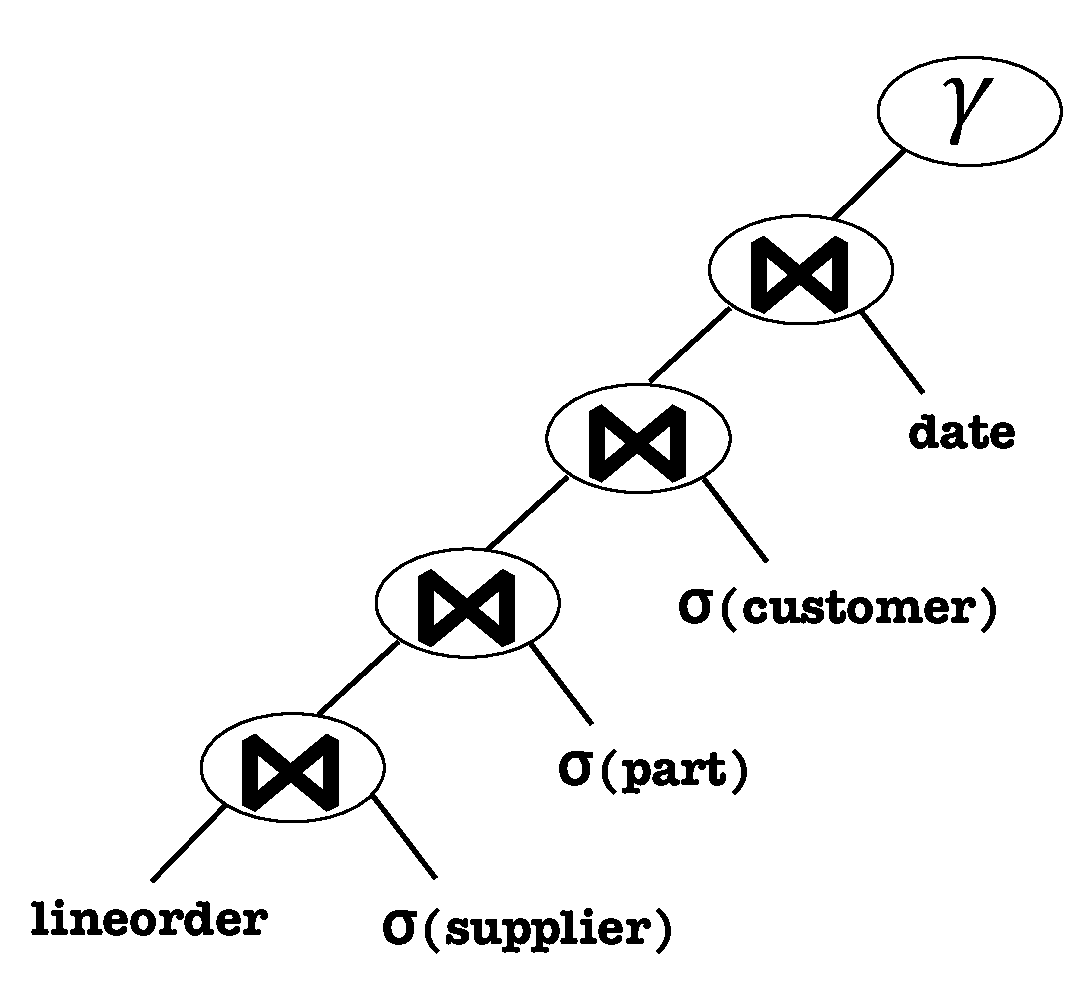
\includegraphics[width=1.0\columnwidth,
                    height=0.75\columnwidth]{pictures/Q41-original.pdf}
   \caption{Original query plan}
   \label{fig-q41-original}
\end{subfigure} %
\begin{subfigure}[bt]{0.33\textwidth}
  \centering
   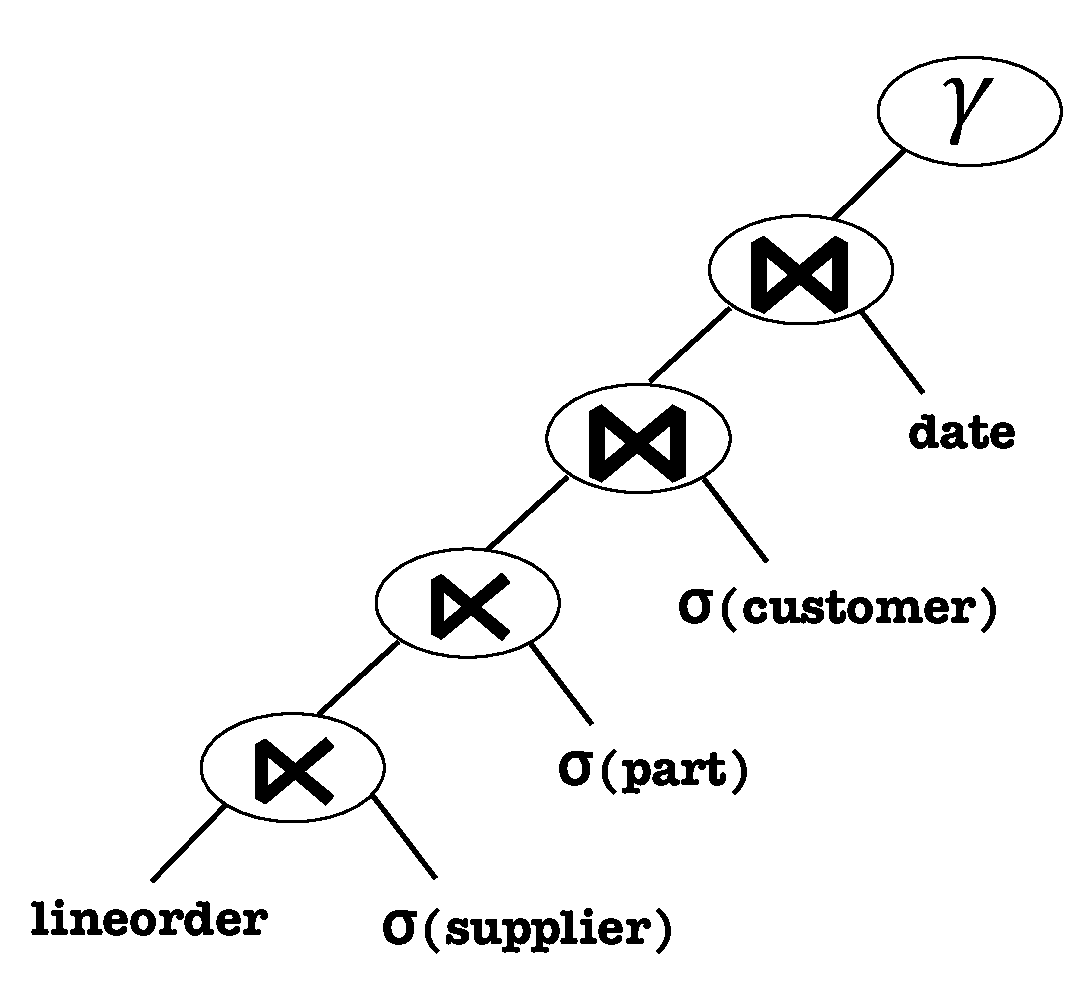
\includegraphics[width=1.0\columnwidth,
                    height=0.75\columnwidth]{pictures/Q41-semijoin.pdf}
   \caption{Plan using join to semi-join transformation}
   \label{fig-q41-semijoin}
\end{subfigure} %
\begin{subfigure}[bt]{0.33\textwidth}
  \centering
   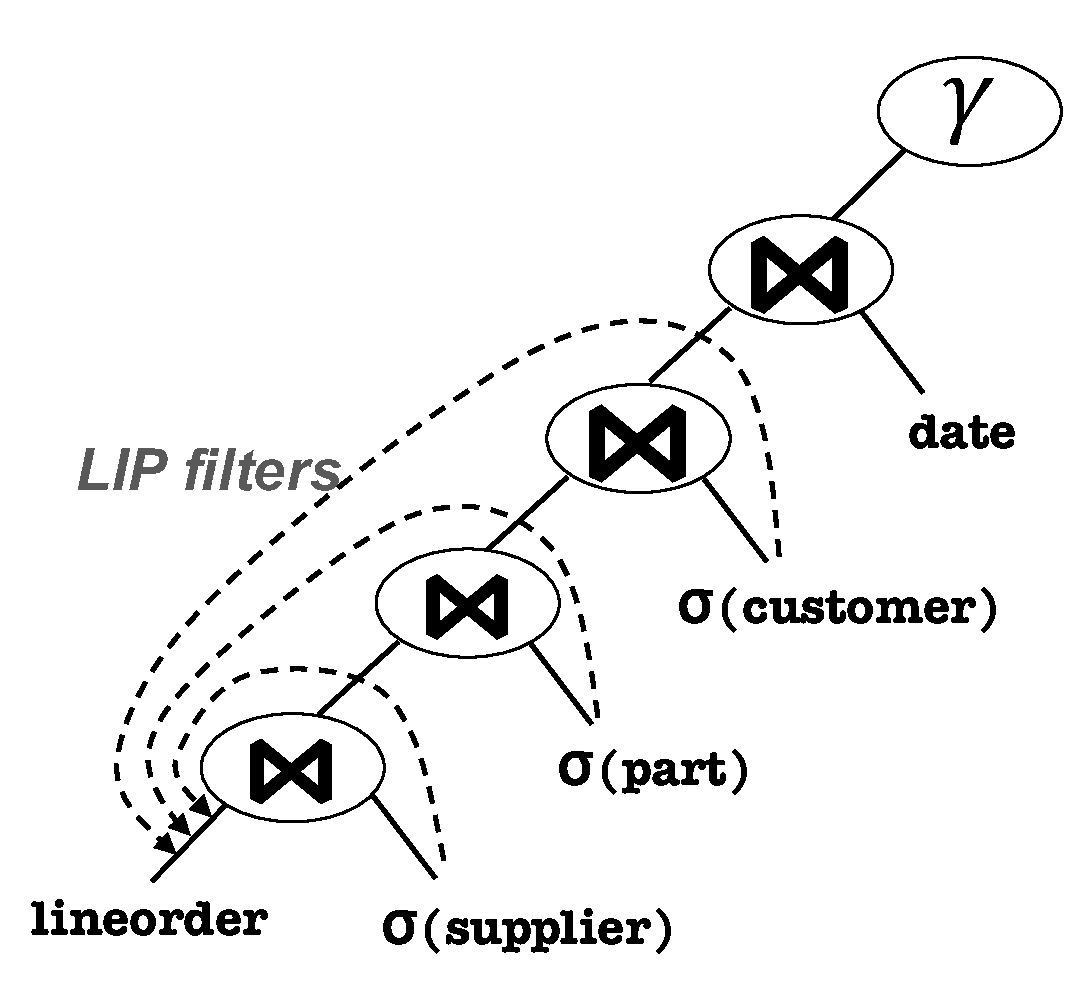
\includegraphics[width=1.0\columnwidth,
                    height=0.75\columnwidth]{pictures/Q41-LIP.pdf}
   \caption{Query plan using LIP (only)}
   \label{fig-q41-lip}
\end{subfigure} %
\caption{\textbf{Query plan variations for SSB Query 4.1}}
\vspace*{2em}
\end{figure*}

Finally, we note that by simply tracking the work orders that are completed, Quickstep can provide a built-in generic query progress monitor (shown in Section~\ref{sec:progress-monitoring}).

%\subsection{TMB} \label{tmb}
%The Transactional Message Bus (TMB for short) is a communication framework designed for scalability (both within a node and across clusters) and reliability~\cite{tmb-full-paper}. Although developed as part of the \Quickstep\ project, it is a fully self-contained and general-purpose framework that can be used in other applications. The TMB provides a general-purpose message bus that maintains a consistent view of clients that are connected to it and a queue of incoming messages on each client's behalf. The message bus is \textit{transactional} in the sense that any action using the bus (e.g. connecting/disconecting, sending or receiving messages, deleting or cancelling messages, etc.) is an ACID transaction on the state of the bus. The semantics of message addressing and delivery are well-defined and based on causal ordering~\cite{causal-multicast}. There are several mutually-compatible implementations of the TMB available, some of which ``piggyback'' on existing transaction-processing systems, as well as a native implementation that consists of a custom in-memory transaction manager and simple write-ahead log for durability and recovery.

%Besides its core responsibility of reliable message delivery between clients, the TMB includes some additional features that are desirable when building a reliable and responsive parallel or distributed system. These include group messaging, separate message reciept and deletion for reliability when clients may fail, and tied messages to mitigate variable latency and work skew~\cite{tail-at-scale}. Because the TMB is itself a kind of database, it can also be queried for informational purposes (e.g. queue lengths can be examined for progress monitoring and straggler detection).


%\subsection{Partitioning} \label{sec-partitioning}
%\Quickstep\ also has the notion of partitioning a table, which is used to control the distribution of data across NUMA memory.
%
%A relation can be partitioned horizontally using either \textit{hash} or \textit{range} partitioning. Both base and temporary relations can be partitioned. Every relation that is partitioned has an associated \textit{partition scheme}. A partition scheme %is implemented internally as a C++ class which
%records the partitioning function, the partitioning attribute(s),
%%the number of partitions,
%and a map of the blocks to each partition.
%
%When tuples are inserted into a relation, the partition scheme determines which partition each tuple belongs to based on its own internal policy (e.g. computing the hash of a particular attribute's value and then computing the remainder modulo the number of partitions), and divides the tuples so that they are inserted into blocks belonging to the appropriate partition. %The partition scheme class defines a generic interface that allows for other partitioning methods besides simple hash and range-based partitioning to be easily added in the future.
%
%%\begin{figure}
%%\centering
%%\includegraphics[width=2.5in]{pictures/numa-optimization}
%%\caption{NUMA optimization}\label{fig-numa}
%%\end{figure}
%
%The following example illustrates hash partitioning, where the hash function for integers is the identity function. Consider a relation R, with a single attribute of type integer, which is also the partitioning attribute. The relation is hash partitioned with 4 partitions. When a tuple with value 0 or 4 is inserted, the tuple is placed in a block belonging to partition 0. When the next tuple with value 1 or 5 is inserted, although there is space left in the block that was previously created, a new block is created since this tuple belongs to partition 1. In a similar way, all the tuples belonging to a particular partition are inserted into blocks that belong to that partition.
%
%When an operator in \Quickstep\ needs to write data to blocks, it uses a class called \textit{InsertDestination}, which has methods for inserting tuples one-at-a-time or in bulk. The InsertDestination interface is responsible for the common tasks of pushing data into blocks, creating new empty blocks as needed, and signaling to the foreman when blocks are full and ready to be consumed.
%InsertDestinations have an associated partition scheme (the default is no partitioning).
%
%When inserting tuples into an InsertDestination, a pass is first made to assign each tuple to a partition (querying the Partition Scheme). Then, tuples are bulk-inserted into blocks belonging to the appropriate partitions, with new blocks being created in each partition when needed. By implementing partitioning as an option in the common tuple-insertion path, we can easily partition relations when data is loaded \textit{or} repartition the output of any operator on-the-fly as part of normal query execution.
%
%To illustrate how partitioning works, consider the following query: % (we also reuse this query later in Section~\ref{eval-numa}): \vspace*{-0.5ex} \reminder{check}
%\begin{verbatim}
%  SELECT p_partkey FROM lineorder JOIN part;
%\end{verbatim} \vspace*{-0.5ex}
%
%%In the query shown in the Section~\ref{eval-numa}, the end-to-end partitioning works as follows:
%Assume that the relations \textsf{lineorder} and \textsf{part} are partitioned into four partitions each, using hash-partitioning on the join key when they are created. When the data is loaded for these relations, each tuple is inserted into a block belonging to the appropriate partition. If the system has four sockets, then each  corresponding partition of both the relations are placed across the four sockets, with one partition-pair per socket. When computing the hash join between these two relations, four hash tables are created, with one per partition-pair across the four (NUMA) sockets. Work orders for both the build and the probe phase of the hash join will access local memory on only one NUMA socket for input blocks, the hash table, and for materializing join output.
%
%The scheduler (described above in Section~\ref{scheduler}) is also NUMA-aware, and
%whenever possible aims to send work orders to the NUMA node where the data referred to in the work order resides.
%
%%aims to send each work order to a worker thread running on the NUMA node where the input blocks referred to in the work order reside. The scheduler can be configured to be \textit{strict} with regard to NUMA-aware scheduling (only giving workers NUMA-local work orders), or to allow a relaxed \textit{work-stealing} policy, where idle workers on other sockets can be assigned non-local work orders at times when there are no NUMA-local work orders for them to process.
%
%\begin{figure*}
%\centering
%\begin{minipage}{.31\textwidth}
%  \centering
%  \includegraphics[width=2.2in]{pictures/elasticity-scan}
%  \caption{Elasticity with a Scan query \newline \newline }
%  \label{fig-elasticity-scan}
%\end{minipage}%
%\quad
%\begin{minipage}{.31\textwidth}
%  \centering
%  \includegraphics[width=2.2in]{pictures/elasticity-join1}
%  \caption{Elasticity with a Join query: Add a second thread mid-way through the build phase}
%  \label{fig-elasticity-join1}
%\end{minipage}%
%\quad
%\begin{minipage}{.31\textwidth}
%  \centering
%  \includegraphics[width=2.2in]{pictures/elasticity-join2}
%  \caption{Elasticity with a Join query: Add a second thread at the end of the build phase}
%  \label{fig-elasticity-join2}
%\end{minipage}
%\end{figure*}

%\subsection{WideTables} \label{sec-widetables}
%\Quickstep\ can also use a schema-based denormalization technique called WideTable~\cite{widetable}. This technique walks through the schema graph of the database, and converts all foreign-key primary-key ``links'' into an outer-join expression (to preserve NULL semantics). The resulting ``flattened'' table is called a WideTable, and is essentially a denormalized view of the entire database. The columns in this WideTable are stored as column-stores, and BitWeaving indices can be additionally built on columns of interest.
%
%This type of denormalization is largely agnostic of workload characteristics (it is a schema-based transformation). It has been acknowledged that such techniques are expensive for databases that are updated often, and our implementation is very rudimentary -- we currently have to recreate the WideTable on updates. Techniques for incrementally updating the WideTable (rather than recreating it from scratch) when new data is appended to existing tables can be envisioned, but we have yet to implement them.
%
%In addition, we have a relatively simple optimizer (recall from Section~\ref{overview} that we have a simple rule-based optimizer) that currently only allows for simple transformation of queries. As a result, only a limited class of queries can be answered for databases on which WideTables are built. Note, that \Quickstep\ does allow running queries using regular joins, so when a WideTable is dropped and has to be reconstructed, the system can still execute queries using traditional methods (although the performance may be lower).
